% Options for packages loaded elsewhere
\PassOptionsToPackage{unicode}{hyperref}
\PassOptionsToPackage{hyphens}{url}
%
\documentclass[10pt,a4paper]{article}
\usepackage[left=25mm,right=25mm]{geometry}
\usepackage{amsmath}
\usepackage{amsfonts}
\usepackage{amssymb}

\author{}
\date{}



\usepackage{listings}
\usepackage{color}

\definecolor{dkgreen}{rgb}{0,0.6,0}
\definecolor{gray}{rgb}{0.5,0.5,0.5}
\definecolor{mauve}{rgb}{0.58,0,0.82}

\lstset{frame=tb,
  language=C,
  aboveskip=3mm,
  belowskip=3mm,
  showstringspaces=false,
  columns=flexible,
  basicstyle={\small\ttfamily},
  numbers=none,
  numberstyle=\tiny\color{gray},
  keywordstyle=\color{blue},
  commentstyle=\color{dkgreen},
  stringstyle=\color{mauve},
  breaklines=true,
  breakatwhitespace=true,
  tabsize=3
}

\usepackage{multicol}
\usepackage{graphicx}
\usepackage{epstopdf}

\epstopdfDeclareGraphicsRule{.gif}{png}{.png}{convert gif:#1 png:\OutputFile}
\AppendGraphicsExtensions{.gif}
\usepackage{chngcntr}
\counterwithin*{equation}{section}
\counterwithin*{equation}{subsection}
\usepackage{amsmath}

\usepackage{float} 
\usepackage{hyperref}
\usepackage{amsmath}
\let\oldsubsection\subsection
\renewcommand{\subsection}{%
    \setcounter{equation}{0}%
    \oldsubsection%
}
\begin{document}


\begin{flushleft}
\begin{LARGE}EE 435 Lab 3 Spring 2024
\end{LARGE}
\\Jonathan Hess and Grant Nordling
\\\href{https://github.com/Jetsama/EE435/tree/main/Labs/Lab3}{GitHub Page}
\end{flushleft}

\begin{LARGE}
Current-Mirror Operational Amplifier Design
\end{LARGE}


The current mirror op amp is shown below. This can be used as a
standard operational amplifier in a feedback configuration though when it
was introduced the primary focus was on using it in open-loop applications
as an Operational Transconductance Amplifier (OTA).

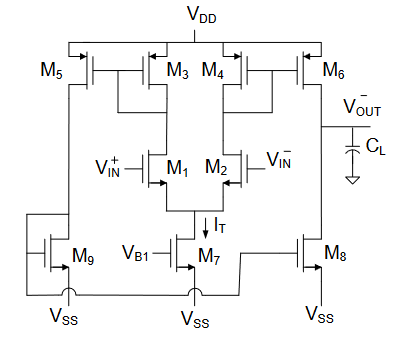
\includegraphics[width=3in]{images/Image1.png} \\


\subsection*{Part 1}
Design this op amp in a 0.18$\mu$m process with supply voltages of
VDD=1.5V and VSS =-1.5V. In this design, the lengths of all devices
should be 5xL min , the mirror gains M 35 and M46 should be 10, the mirror
gain M98 should be 1, the power dissipation should be 1mW, and V EB
should be 100mV for all devices.


The first step taken wss to figure how the constraints affected the design.

Using the power constraint ($P = 1mW$) we can constrain the current because the $P = IV$. Voltage is $VDD-VSS = 3V$, this means current equals 333.33$\mu$A. Because of the current mirrors and symmetry we can find the tail current. The paths are laid out like so. 


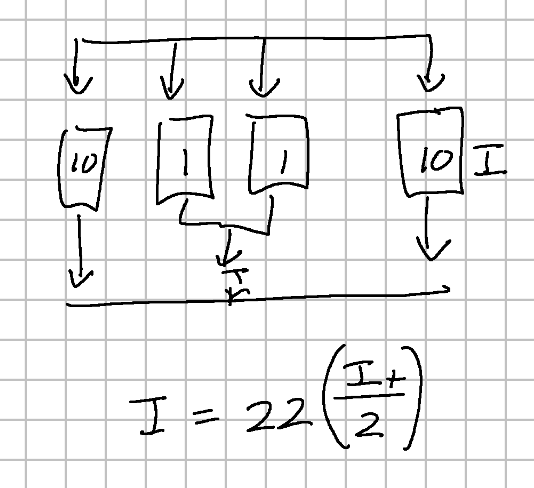
\includegraphics[width=3in]{images/Image2.png} \\


The tail current is $\frac{(333.33\mu A)}{11} = 30.30\mu A$ and because the bias current has been constrained as well we can solve for the W/L ratio.\\

Using the DC operating point we can find the VTH and other process parameters.\\
$M3 = M4 = (1/10) * M5 = (1/10) * M6$\\
$M1 = M2$\\
$M7 = $ fixed due to power\\
$M9 = M8$\\

\subsection*{Part 2}
Analytically determine the differential voltage gain, the BW, the GB,
and the SR of this amplifier. Assume CL =20pF\\


The gain, bandwidth, gain bandwidth, and slew rate can be determined by the following equations given in the lecture slides.\\

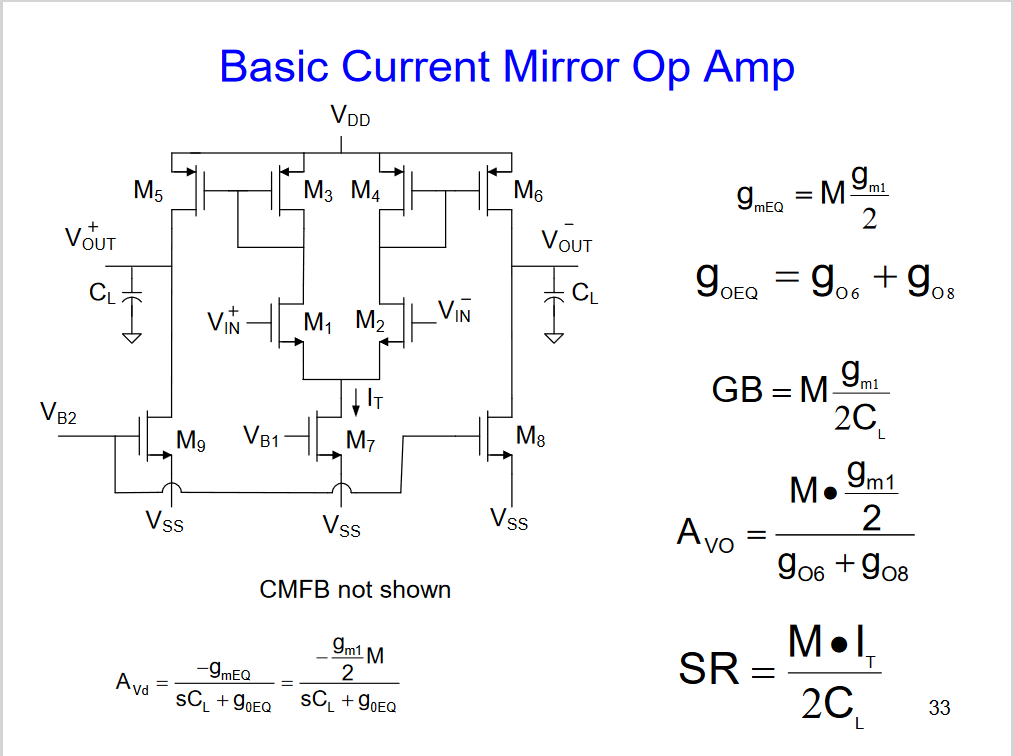
\includegraphics[width=3in]{images/Char.png} \\
Where M is the value of the current mirror (10) $C_L$ is the load capacitor, and gm1 is the gain of the m1/m2 mosfet. 

This means that using our values provided so far:\\
$A = \frac{10*gm_1}{g_6+g_8}$ \\
$BW = \frac{GB}{A}$ \\
$GB = 10 * \frac{gm_1}{2*20pF}$ \\
$SR = \frac{10*30.30\mu A}{2*20pF}$ \\


We set the width to length ratio for M1 to 100 and  


\subsection*{Part 3}
Analytically determine the output signal swing for a common-mode
input of -200mV

First step was to determine the width to length values. Lambda is the Channel length modulation parameter. This was done with a simple test bench containing one transistor.\\



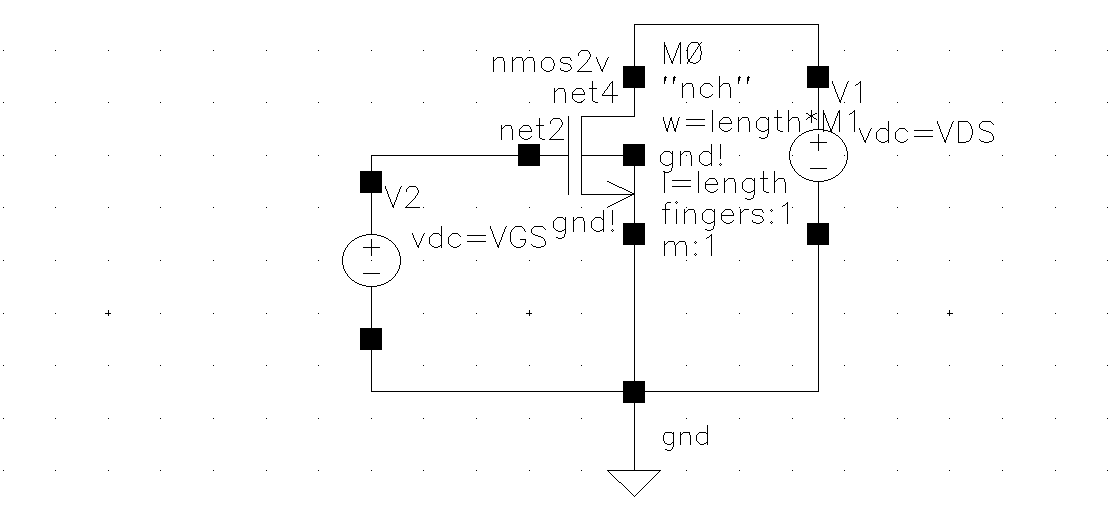
\includegraphics[width=3in]{images/mosTB.png} \\

The equations used to create find these values are as follows:

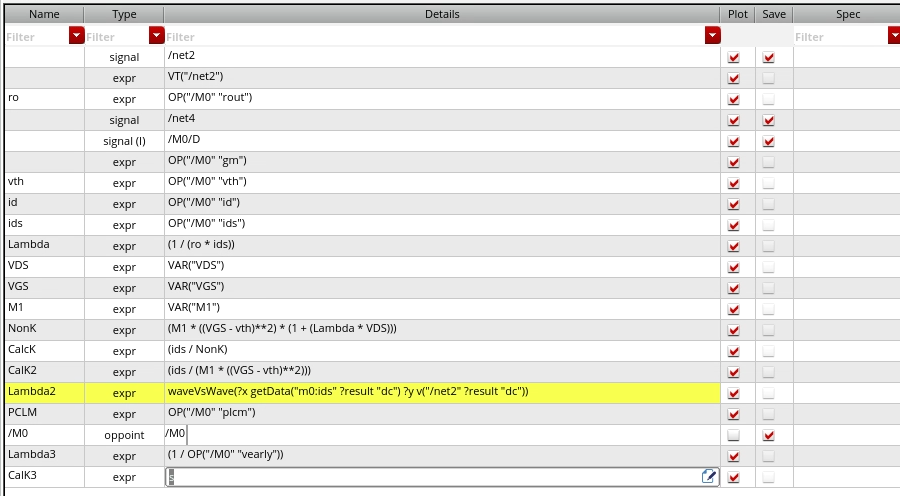
\includegraphics[width=6in]{images/mosTBEQ.png} \\

What is concering is that despite having a constant VGS and accounting for VDS changes with lambda we still see this curve in the constant K value.\\
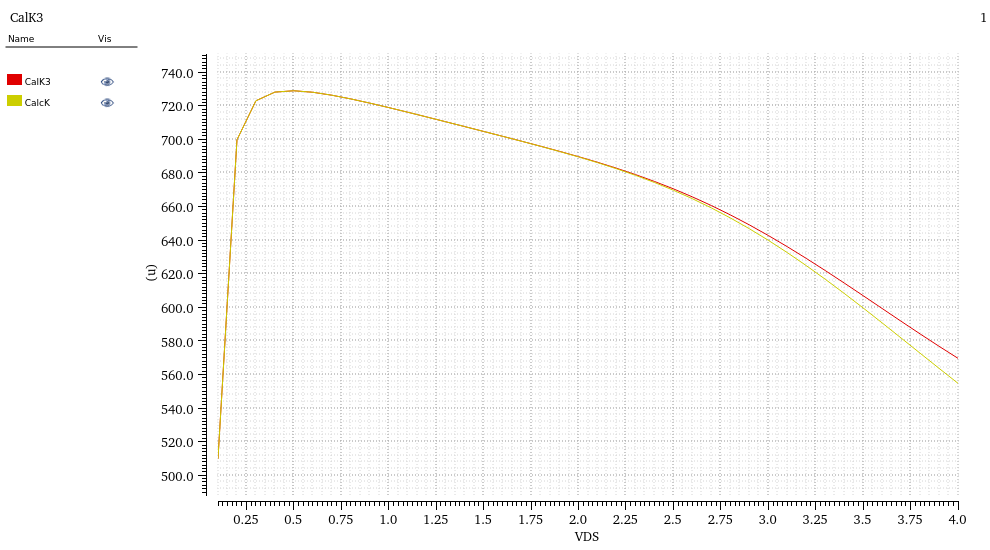
\includegraphics[width=3in]{images/Lambda23.png} \\



\subsection*{Part 4}
Compare the results obtained in part 2 and part 3 with computer
simulations.

Because of the model we used in the lab the simple saturation model for the transistor was not accurate. We had to edit our width to length to 8. 

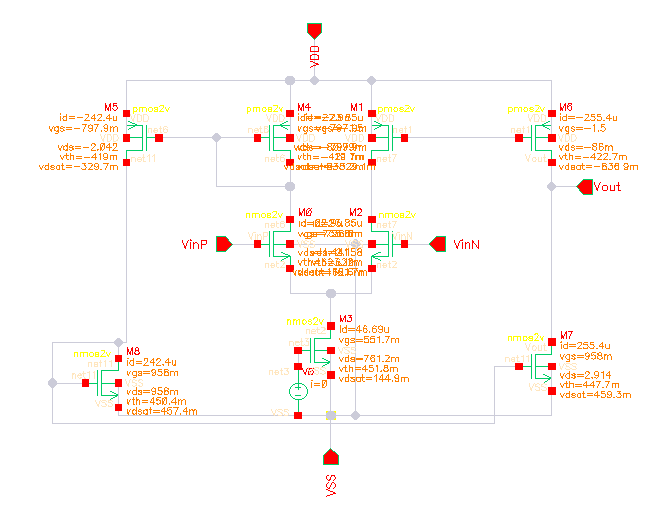
\includegraphics[width=3in]{images/Design.png} \\


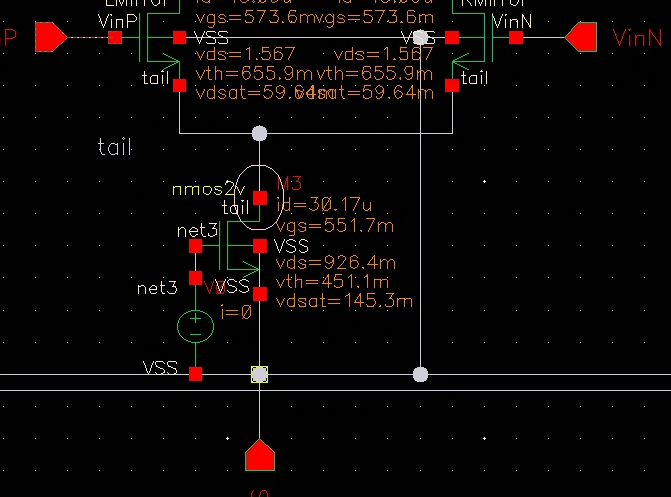
\includegraphics[width=3in]{images/tailcurrent.png} \\

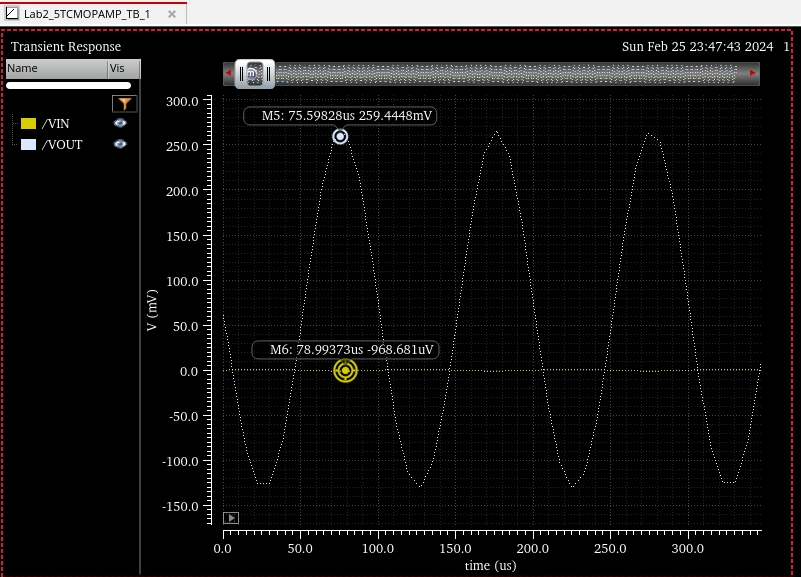
\includegraphics[width=3in]{images/output.png} \\



\subsection*{Part 5}
What is the 3dB bandwidth when feedback is applied to form a unity-
gain buffer?

\subsection*{Part 6}
What is the response of the unity-gain feedback amplifier to a 100mV
step input with a common-mode input of -200mV?


At first I used a sine wave with 200mv swing without unity gain.\\
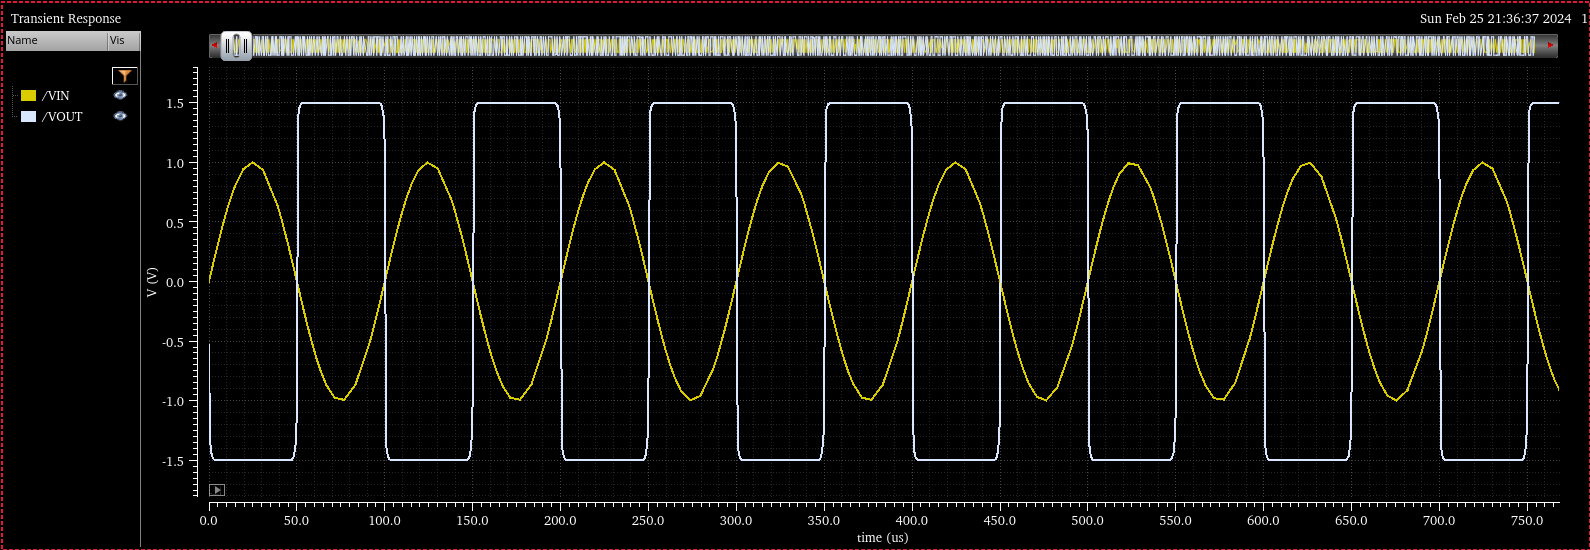
\includegraphics[width=3in]{images/attempt1200mv.png} \\

After fixing the testbench and using a input of -200mV the graph had a unity gain\\

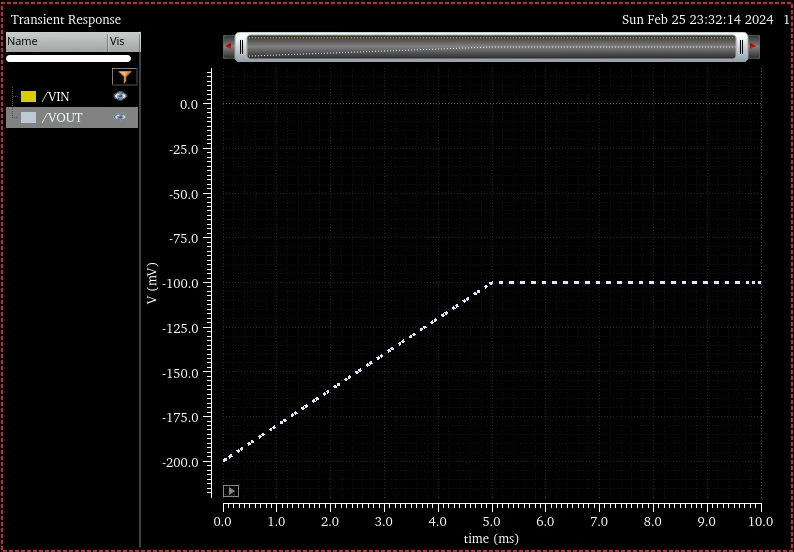
\includegraphics[width=3in]{images/attempt2200mv.png} \\

\subsection*{Part 7}
Determine the poles and zeros using a Spice analysis for both the
open-loop and closed-loop amplifier. The feedback should provide a
dc gain of +1. Plot the two dominant open-loop and closed-loop poles

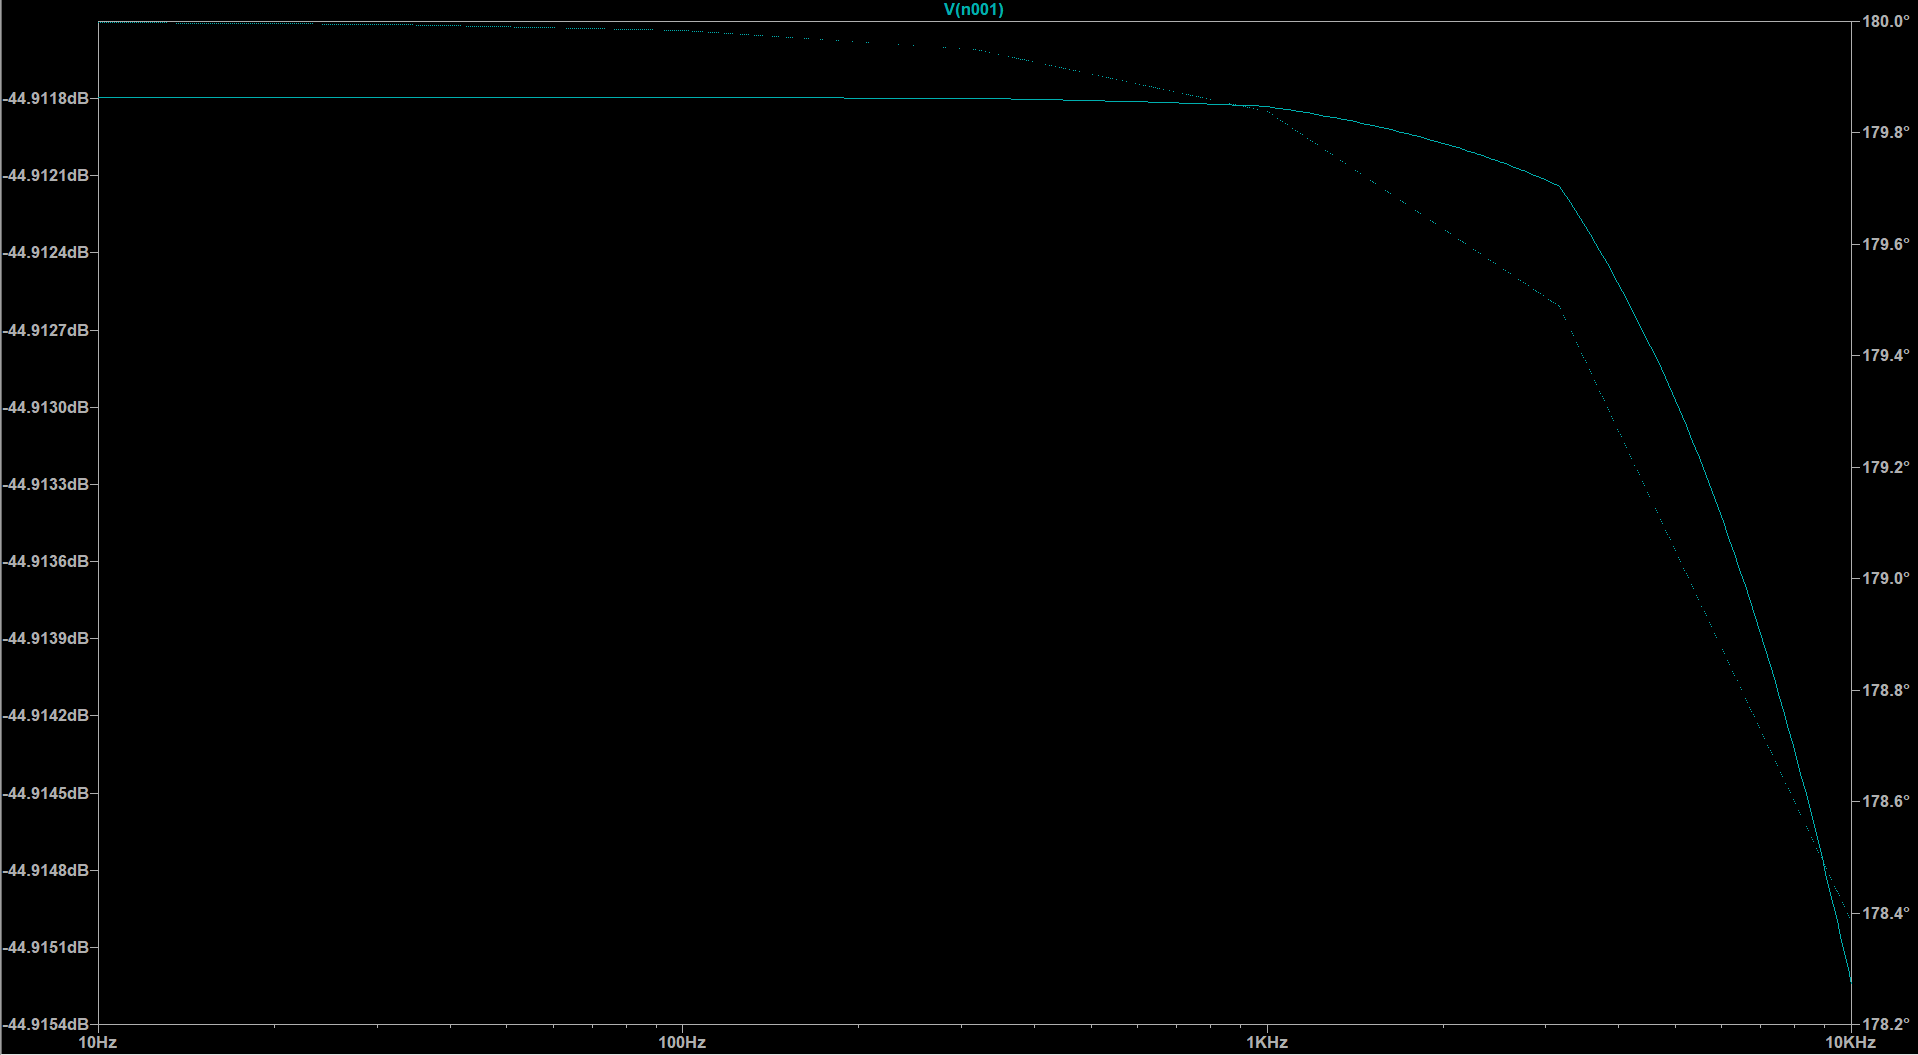
\includegraphics[width=3in]{images/spice.png} \\

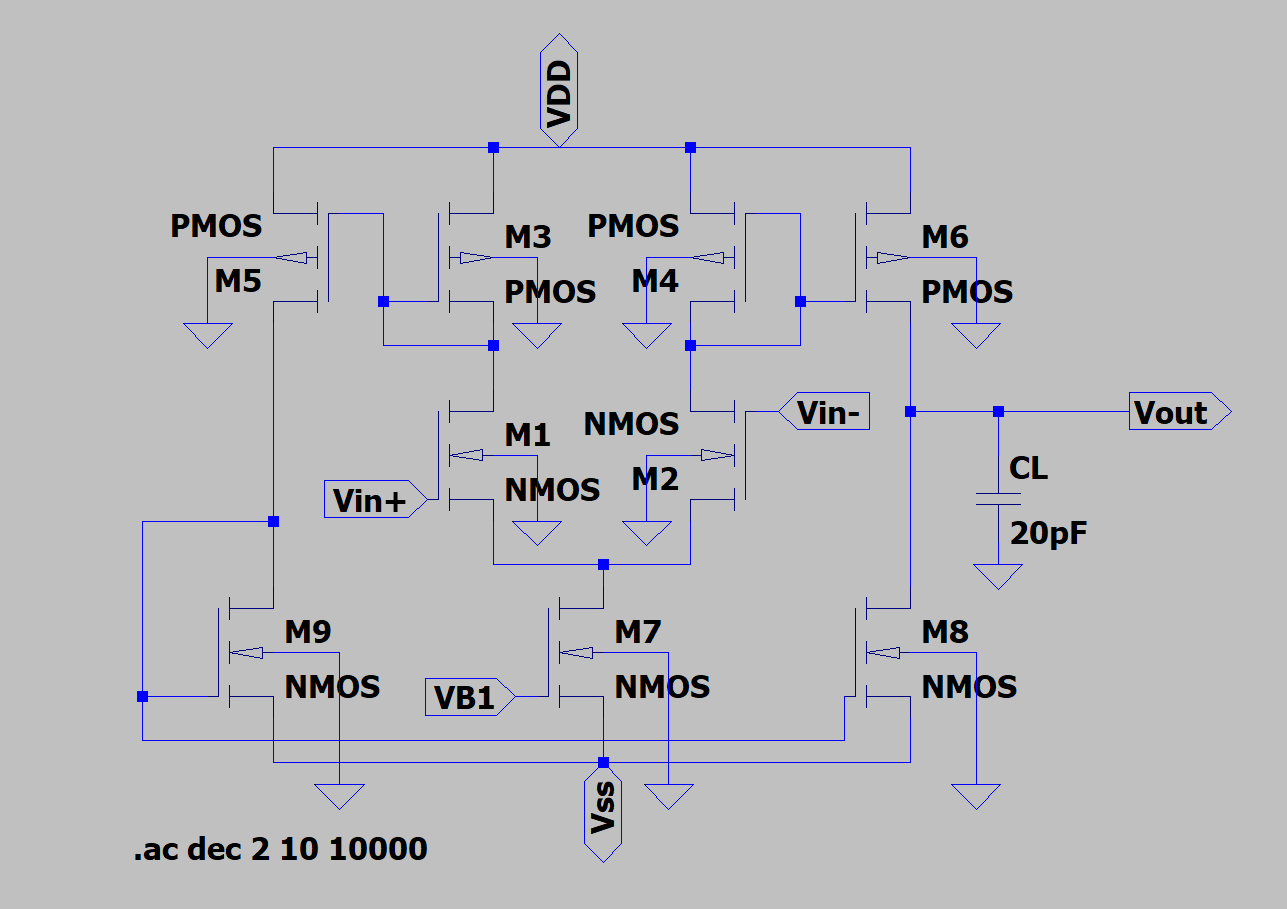
\includegraphics[width=3in]{images/7TLTspice.png} \\


\end{document}
